\chapter{Implementation}
% Main diagram of the entire system

\section{Tool Choice}
\label{sec:tool_choice}

\subsection{C++ with a Separate Tool}
\begin{figure}[h!]
    \centering
    \includegraphics[scale=1]{implementation/_diagrams/clang_comptime.pdf}
    \caption{Clang Compiler Pipeline}
\end{figure}
\noindent
Due to the lack of unification on build systems, and the lack of support for abstractions powerful enough to do schema compilation at compile time in C++, an external tool invocable on schema files is required.
\begin{itemize}
    \setlength\itemsep{0em}
    \item C++ has powerful metaprogramming capabilities for building the data structures to be used by the database implementation.
    \item Substantial tooling (profilers, debuggers) available.
    \item Some analysis of embedded C++ code can be done using clang libtools (much like clang static-analyzer \& clang tidy), but propagation of error messages is difficult.
    \item Without additional tools being developed, language server/IDE support is impossible.
\end{itemize}

\subsection{Zig Comptime}
\begin{figure}[h!]
    \centering
    \includegraphics[scale=1]{implementation/_diagrams/zig_comptime.pdf}
    \caption{Zig Compiler Pipeline}
\end{figure}
\noindent
Zig supports compile time reflection and code execution. It is a far more powerful and complete
implementation than those currently present in C++23'S \mintinline{cpp}{constexpr} \&\mintinline{cpp}{consteval},
or Rust's \mintinline{rust}{const} generics.
\begin{center}
    \begin{tabular}{l p{.8\textwidth}}
        \textbf{comptime} & Types are values, can be assigned, passed, and have data structures, functions generated, can pass errors to the compiler. Restrictions on IO. \\
        \textbf{runtime} & Types erased, access only to non-comptime values.                                                                                              \\
    \end{tabular}
\end{center}
Rather than parsing, we allow users to construct comptime structs that describe the operations of
queries, and tables.
\\
\\ At comptime these can be passed to a function, which analyses the structure and can then generate a structure that implements the database.
\begin{itemize}
    \setlength\itemsep{0em}
    \item Limitations on flexibility, produced plans need to be constructed as valid zig datastructures, and implement some method for \textit{execute given query}.
    \item Limited interaction with non-zig code, for example generating plan debug diagrams, or epresentations that can be easily debugged.
    \item Error messages can be made by the library, but are managed by zig, so while expression errors are trivial and managed entirely by zig, assigning spans to certain structures using the query language semantics is difficult.
\end{itemize}

\subsection{Rust Procedural Macros}
\begin{figure}[h!]
    \centering
    \includegraphics[scale=1]{implementation/_diagrams/rust_comptime.pdf}
    \caption{Rust Compiler Pipeline}
\end{figure}
\noindent
Procedural macros are functions which take rust compiler provided tokenstreams as input, and return rust tokenstreams as output and run at compile time. They can interact with the compiler, and the environment (file system, network).
\begin{itemize}
    \setlength\itemsep{0em}
    \item They are a key language feature of rust, and are ubiqutous across the rust standard library and ecosystem.
    \item They can contain arbitrary code, which includes a schema compiler.
    \item The tokens provided to proc macros are basic tokens (identifiers/words, punctuation, literals, brackets), and do not have to conform to rust syntax.
\end{itemize}
Rust proc macros can also generate error messages and output code, using spans from the original tokens.
\begin{itemize}
    \setlength\itemsep{0em}
    \item Rust reports error diagnostics from rust, alongside errors generated by procedural macros (meaning they are also passed to the language server and displayed in IDE).
    \item User code passed through to generated code by macros retain their original spans, so errors can attributed to user code in their original position.
\end{itemize}
\begin{figure}[h!]
    \centering
    \includegraphics[width=\textwidth]{implementation/_diagrams/rust_proc_macro.pdf}
    \caption{Procedural Macros in the Rust Build System}
\end{figure}

\subsection{Decision}
\begin{center}
    \begin{tabular}{l l | l l l l}
        & & \multicolumn{4}{c}{\textbf{Tool}} \\
        & \textbf{Feature}                         & zig  & rust & tool $\to$ cpp & scala \\
        \hline
        & Custom Syntax     & No   & Yes  & Yes            & Yes   \\
        & Error Propagation & Yes  & Yes  & No             & Yes   \\
        \textbf{Requirement} & Performance       & Good & Good & Good           & Poor  \\
    \end{tabular}
\end{center}
\begin{itemize}
    \setlength\itemsep{0em}
    \item Rust's support for lifetime-bound references is particularly advantageous in the context of returning references to immutable data.
    \item Rust's safety features make generating code far safer than zig, or C++.
    \item Existing support for parsing rust ASTs allow for easier development of the schema compiler.
    \item Zig does not allow IO at comptime, so generating diagrams, or other debug information separate from code is difficult.
    \item Other languages supporting code generation (in particular scala 3 macros) were not considered due to lacking performance (garbage collection).
\end{itemize}
Hence the chosen option was a rust procedural macro.

\section{System Overview}
\begin{figure}[h!]
    \centering
    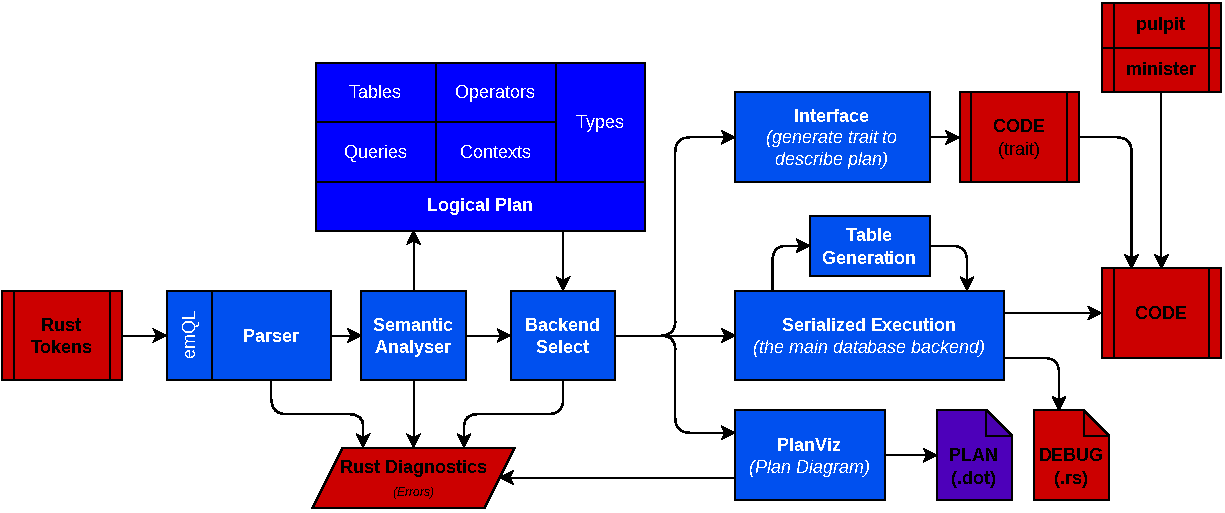
\includegraphics[width=\textwidth]{implementation/_diagrams/system.pdf}
    \caption{System Design}
\end{figure}
\noindent
Given the limited time, and the requirement to complete the entire end-to-end compilation in order to test optimisations:
\begin{itemize}
    \setlength\itemsep{0em}
    \item Implement only the mutable\ref{sec:app_opt} \& append only\ref{sec:mut_opt} optimisations.
    \item Build the system to be easily extendable (need to support multiple backends, and have a backend-agnostic logical plan).
    \item Rather than implementing and optimising a small subset of functionality, to implement all functionality required for a database and use the remaining time for optimisation.
\end{itemize}


\section{Language Design}
In deciding the query language for any database, SQL was a natural choice.
\begin{center}
    \begin{tabular}{l l | l l l l}
                          &                                   & \multicolumn{4}{c}{\textbf{Language}}                                 \\
                          & \textbf{Feature}                  & SQL                                   & SQL rustified & flux & custom \\
        \hline
                          & SQL Compliant (Tooling)           & Yes                                   & No            & No   & No     \\
        \textbf{required} & Compatible with rust types        & No                                    & Yes           & No   & Yes    \\
        \textbf{required} & Compatible with rust expressions  & No                                    & Yes           & No   & Yes    \\
                          & Rust Syntax Shadowed Highlighting & No                                    & No            & Yes  & Yes    \\
    \end{tabular}
\end{center}
\noindent
Embedding rust expressions and types into the database avoids a costly (query language) $\to$ rust translation
requirement, and allows for simple embedding of application code.
\subsection{emQL Overview}
The emQL language developed for this project is inspired by both the flux language syntax, and by iterators (specifically the \mintinline{elixir}{|>} elixir pipe).
\begin{itemize}
    \setlength\itemsep{0em}
    \item Queries are directed acyclical graphs (DAGs). Unlike SQL which represents queries (with some exceptions\footnote{Recursive Common Table Expressions})
          as trees, emQL allows for streams to me merged, forked, and have stream elements be individually lifted
          into a subcontext (another DAG inside a query DAG).
    \item Operators are ordered by dataflow (\mintinline{rust}{op1 |> op2 |> op3}), rather than by operation
          (SQL requires a rigid ordering of \mintinline{SQL}{SELECT .. FROM .. WHERE .. }). This means that queries
          can be written in a more concise, and more intutive imperative style.
    \item Row references are a core concept in emQL. They are fast lookup keys into tables that are used in
          \mintinline{rust}{update} and \mintinline{rust}{delete} operations and are provided by \mintinline{rust}{insert},
          \mintinline{rust}{ref} and \mintinline{rust}{unique} operations. As row references are just data, they can be mapped,
          processed and acted on by user logic, and are stable so can be sent \& stored outside the database for use in fast
          lookups later. Row references are a significant performance advantage for OLTP workloads that allow the database to
          select a unique identifier.
    \item Mutable and ure operations mixed. Rather than requiring separate \mintinline{rust}{SELECT} and \mintinline{rust}{UPDATE}
          operations, emQL allows for a single query to both read and write data in a single pipeline of operators on a stream.
          This allows for more concise queries.
    \item All queries are just transactions. Though they are called \mintinline{rust}{query}, emQL queries are equivalent to SQL
          transactions with potentially many operations.
    \item Reference types are explicit at accessed using \mintinline{rust}{'qy} and \mintinline{rust}{'db}. The backend chooses the types provided by \mintinline{rust}{deref} and \mintinline{rust}{use}
          during table selection, and can optimise these. The chosen types are exposed to the user so they can decide to for example (use
          \mintinline{rust}{Cow} on an immutable reference rather than cloning when mapping with mutation).
\end{itemize}
For example the following schema is valid emQL from .
\begin{minted}{rust}
impl my_db as Serialized { 
    // options can be specified for implementations
    aggressive_inlining = on,
};

table people {
    name: String,
    birth_year: u16,
    friend: Option<String>,
} @ [
\end{minted}
Constraints can be applied for unique columns, table length limit and row predicates. The provided names are used in the error return types on constraint breach
\begin{minted}{rust}
    unique(name) as unique_names, 
    limit(1000) as max_people, 
    pred(name.len() < 100) as sensible_name_length 
]
\end{minted}
Each query is expressed as a method on the generated database object
\begin{itemize}
    \setlength\itemsep{0em}
    \item The self borrow is determined by the mutation operations in the query
    \item The return type is inferred from the query, and is free for the backend to make optimisation decisions on.
\end{itemize}
\begin{minted}{rust}
// DESCRIPTION: Get the number of friendships between people born in the same decade
query same_year_friendships() {
    use people 
        |> map(
            name: &'db String = name, 
            birth_decade: u16 = (birth_year / 10) * 10,
            friend: &'db Option<String> = friend
        )
        |> groupby(birth_decade for let same_year_people in {
            // Queries are not nested like SQL, but are a DAG, streams can be duplicated.
            use same_year_people |> fork(let friend_side, friended_side);

            join(use friend_side [
                // predicate (inner), cross and equi (inner) joins are supported
                inner pred { 
                    if let Some(friend_name) = &left.friend {
                        friend_name == right.name
                    } else {
                        false
                    }
                }
            ] use friended_side)
                |> count(num_friendships)
                ~> map(decade: u16 = birth_decade, num_friendships: usize = num_friendships)
                ~> return;
            }
        )
        |> collect(decades)
        ~> return; // The return type is inferred and includes the errors that can occur.
}

// DESCRIPTION: update an incorrect birth year using a name, and return a row reference
query fix_birth_year(name: &'qy String, new_year: u16) {
    row(
        // using a reference type for input ('qy is the lifetime of the borrow of the database)
        name: &'qy String = name,
    )
        ~> unique(name for people.name as ref person) // access to columns with unique indexes
        ~> update(person use birth_year = new_year)
        ~> map(person: ref people = person) // use of a row reference type
        ~> return;
}

// DESCRIPTION: Add a new person, and return the number of people who declare them a friend. 
query new_friendship(user_name: &str, friend: Option<String>) {
    row(
        name: String = String::from(user_name),
        friend: Option<String> = friend,
        birth_year: u16 = crate::CURRENT_YEAR,
    )
        ~> insert(people as ref new_person_id)
        ~> let person_id; // streams and singles can be assigned to (single read) variables.
    
\end{minted}
The lift operator opens a new context, with the stream/single's record fields
available to use in expressions, here it means we can refer to \mintinline{rust}{new_person_id}
in an expression, while also using \mintinline{rust}{user_name} from the query's top context
\begin{minted}{rust}
    use person_id
        ~> lift(
            ref people as other_person_id
                    // access with a row reference to the column `friend`
                |> deref(other_person_id as other_person use friend)
                |> filter(
                    if let Some(other_name) = &other_person.friend { 
                        other_name == user_name && *other_person_id != new_person_id 
                    } else {
                        false 
                    })
                |> count(current_frienders)
                ~> return;
        ) ~> return;
}
\end{minted}

\begin{futurebox}{Stream in and out}
    emQL queries are currently limited to taking in values (singles) and returning single values.
    \begin{itemize}
        \setlength\itemsep{0em}
        \item Allowing queries to consume streams requires modifying the interface to take a struct argument with the specified fields.
        \item Returning streams without collecting values is more difficult, and requires allowing records to contain a variable number of generic parameters for the types of contained streams, implementing some trait (for example \mintinline{rust}{impl Iterator<Item=T>}).
    \end{itemize}
    This feature would preventremove the requirement for immediate collection before return (some potential performance benefits if users intend to iterate over results), and for flattening nested streams (rather than collecting to \mintinline{rust}{Vec}, and then concatenating them - expensive).
\end{futurebox}
\begin{futurebox}{Subqueries}
    Subqueries can be enabled by connecting a \mintinline{rust}{call} operator to the context used by the other query. The semantic analysis however requires the called query's return type to be known.
    This requires significant modifcation to the current semantic analyser to track incomplete analyses, and must include a restriction on recursive (or even mutually recursive) queries.
\end{futurebox}
\section{Query Parsing with Combi}
\subsection{Rust Tokenstreams}
Rust procedural macros can access tokens provided by the rust compiler through the compiler provided \mintinline{rust}{proc_macro} crate.
\begin{itemize}
    \setlength\itemsep{0em}
    \item The \mintinline{rust}{proc_macro} crate provides a stable interface for tokens which are indexes into an AST held in compiler memory.
    \item The \mintinline{rust}{proc_macro2} crate provides a wrapper for \mintinline{rust}{proc_macro} types to allow them to be used outside of a procedural macro context (for example in unit tests).
\end{itemize}
\begin{figure}[h!]
    \centering
    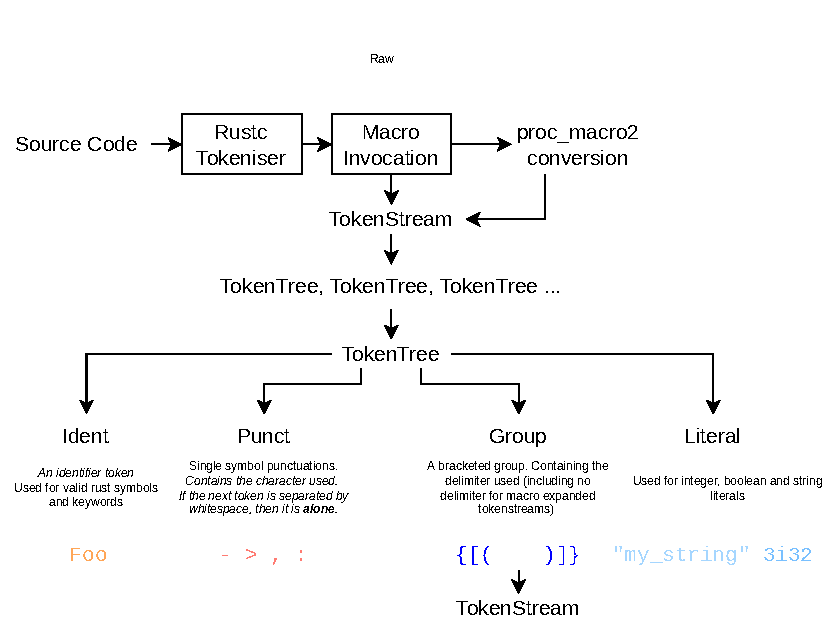
\includegraphics[width=\textwidth]{implementation/_diagrams/tokenstreams.pdf}
    \caption{Rust Tokenstreams}
\end{figure}
\noindent
Each tokentree and tokenstream is associated with a \mintinline{rust}{Span} which tracks its original file \& position,
and can be used in generating diagnostics (spans used to highlight in error messages, and by the language server for highlighting in IDE).
\subsection{Tokenstream Parsers}
The parser used needs to either unfold the tokenstream, or be able to parse tree data structures.
\begin{itemize}
    \setlength\itemsep{0em}
    \item Unfolding the tree is expensive, and can loose some information (for example brackets are associated with spans for open close)
    \item Parsing a tree is not supported by most parser generators, and requires carful management of spans (for example reporting parent error spans when descending into an empty tokenstream).
\end{itemize}
One additional requirement for emQL was to be capable of producing multiple syntax errors, more errors ensures a better development experience. Currently there are only a few parser combinator libraries that can complete this task:
\begin{center}
    \begin{tabular}{l l | l l l l }
                          &                         & \multicolumn{4}{c}{\textbf{Parser}}                                   \\
                          & \textbf{Feature}        & Nom                                 & Chumsky & Chumksy-proc & Winnow \\
        \hline
        \textbf{required} & Multiple Syntax Error   & Manual                              & Yes     & Yes          & Manual \\
        \textbf{required} & Tokenstreams Parsable   & Yes                                 & Yes     & Yes          & Yes    \\
                          & Tokenstream Combinators & No                                  & No      & Yes          & No     \\
                          & Actively Maintained     & Yes                                 & Yes     & No           & Yes    \\
                          & Performance             & Good                                & Poor    & Poor         & Good   \\
    \end{tabular}
\end{center}
\noindent
The only library meeting requirements was chumsky-proc, rather than modify and build atop this library I decided to go for a custom solution, \textit{Combi}.

\subsection{Combi Combinators}
\begin{figure}[h!]
    \centering
    \includegraphics[width=.9\textwidth]{implementation/_diagrams/combi.pdf}
    \caption{Combi Combinators}
\end{figure}
\noindent
The core trait of the library is Combi, it is used to express parsers and recovery mechanisms.
\begin{minted}{rust}
pub trait Combi {
    type Suc;
    type Err;
    type Con;
\end{minted}
Unlike typical parser combinator libraries, the input and output types are independent. This allows for combinators such as \mintinline{rust}{terminal} which convert \mintinline{rust}{TokenStream} $\to$ \mintinline{rust}{()}
\begin{minted}{rust}
    type Inp;
    type Out;
\end{minted}
Apply the computation encoded by the \mintinline{rust}{Combi} on some input data.
\begin{minted}{rust}
    fn comp(&self, input: Self::Inp) -> (Self::Out, CombiResult<Self::Suc, Self::Con, Self::Err>);
\end{minted}
A helper method for describing a combinator (useful in debug messages and for expected error output).
\begin{minted}{rust}
    fn repr(&self, f: &mut Formatter<'_>) -> Result<(), Error>;
}
\end{minted}
Rust token parsing combinators are implemented atop a group of generic core combinators (such as \mintinline{rust}{seq} (sequence two combis), \mintinline{rust}{nothing}, \mintinline{rust}{mapsuc}(map a combinator's success value) and \mintinline{rust}{recursive}).
\begin{itemize}
    \setlength\itemsep{0em}
    \item Additional derived parsers include \mintinline{rust}{listseptrailing}, and the \mintinline{rust}{Fields} builder which generate combinators that parse a set of options (with embedded semantic checks for duplicate, optional, must and default choices), without needing to implement any new combi combinators.
    \item Error embelishment is also included for wrapping errors in expectation messages, based on the structure of combis, and for rewriting
\end{itemize}
\subsection{Performance}
A generated tokenstream (see repository for details) was applied to each parser. All parsers should succeed for all inputs however they have different error capabilities.
\begin{center}
    \begin{tabular}{l p{.8\textwidth}}
        \textbf{Handrolled}   & Panic on failure. Best possible performance at the cost of any error generation.                   \\
        \textbf{Chumsky-Proc} & Attempt to parse, includes error generation, no recovery.                                          \\
        \textbf{Combi}        & Full error recovery for brackets / multiple syntax errors for brackets, includes error generation. \\
    \end{tabular}
\end{center}
\begin{figure}[h!]
    \centering
    \vspace{-0.4em}
    \resizebox{\textwidth}{!}{\input{evaluation/_graphs/tokens.pgf}}
    \caption{Comparative Benchmarks}
\end{figure}
Unsurprisingly the best performance is for the hand-written, panicking parser.  However Combi demonstrates a significant performance advantage over Chumsky-Proc.
\\
\\ Combi's versatility is evidenced by its use for the emDB's emQL frontend, pulpit's table generation macro, and enumtrait's option parsing.
\section{Table Generation with Pulpit}

\subsection{Window Pattern}
\label{sec:window_pattern}
In order to provide mutability optimisation, we need to be able to provide a safe interface to store.
\begin{center}
    \begin{tabular}{l p{.8\textwidth}}
        \textbf{Immutable} & Borrows can last lifetime of object, and are independent from borrows of the mutable side \\
        \textbf{Mutable}   & Normal borrow rules apply                                                                 \\
    \end{tabular}
\end{center}
In order to get a lifetime with which to bind references to the immutable part, we use a \textit{window pattern}.
\begin{figure}[h!]
    \centering
    \includegraphics[width=\textwidth]{implementation/_diagrams/window_pattern.pdf}
    \caption{Window Pattern}
\end{figure}
\subsubsection{Valid Simultaneous Borrows}
\begin{minted}{rust}
let mut val = Value{imm_data, mut_data};
let mut window = ValueWindow::new_window(&mut val);
let (imm_ref, imm_mut_ref) = window.brw();
let mut_ref = window.brw_mut();

let imm_available = imm_ref; // still available
let mut_available = mut_ref; // new mutable taken over from imm_mut_ref
\end{minted}

\subsubsection{Conflicting borrows on the mutable side}
This demonstrates borrow checking working properly still, but for the mutable member.
\begin{minted}{rust}
let mut val = Value{imm_data, mut_data};
let mut window = ValueWindow::new_window(&mut val);
let (imm_ref, imm_mut_ref) = window.brw();
let mut_ref = window.brw_mut(); // ERROR! borrow of mut_ref not possible as imm_mut_ref used later

let value_imm = imm_ref; // still available
let old_mut_unavailable = imm_mut_ref;  
\end{minted}

\subsubsection{No Dangling references}
\begin{minted}{rust}
let imm_ref_dangling;
{
    let mut val = Value{imm_data, mut_data};
    // ERROR! needs to borrow long enough for imm_ref_dangling, but val does not live that long
    let mut window = ValueWindow::new_window(&mut val);
    
    let (imm_ref, imm_mut_ref) = window.brw();
    let mut_ref = window.brw_mut();
    
    imm_ref_dangling = imm_ref;
}
let imm_ref_dangling_unavailable = imm_ref_dangling;
\end{minted}
\begin{center}
    \begin{tabular}{l l l l}
    \end{tabular}
\end{center}

\subsection{Table Structure}
\begin{figure}[h!]
    \centering
    \includegraphics[width=\textwidth]{implementation/_diagrams/table_structure.pdf}
    \caption{Pulpit Table Generation}
\end{figure}
\begin{center}
    \begin{tabular}{l p{.8\textwidth}}
        \textbf{Flexible Design}     & Can be easily configured to support new column data structures, and new selectors.                                                                                                                                                                                          \\
        \textbf{Row vs Column Store} & For emDB an n-ary selector is used, however it is also possible to configure selectors to store data separately from the keys, or to spread data across several columns (decomposed storage).                                                                               \\
        \textbf{Transactions}        & Required for emDB queries, a simple rollback log is used. Due to the support for row references, deletion operations do not drop data or free indices (just ide the row) until commit if trnasactions are enabled to prevent insertions during the commit redusing indices. \\
        \textbf{Precise Errors}      & The return types of methods are constrained to only include possible errors (rather than a generalised error type). This allows for easy matching on errors, and for some operations (such as insert) to have their error type removed when no constraints can be violated. \\
    \end{tabular}
\end{center}
\subsubsection{Side Effects of Clone}
\label{sec:clone_side_effects}
When using a \mintinline{rust}{get}, to get a mutable value from a column the value is cloned.
\begin{itemize}
    \setlength\itemsep{0em}
    \item Pulpit generates clones only for these columns (and as a result needs a separate \mintinline{rust}{Ok(Values { .. })} return type for each get method).
    \item Rust does not eliminate redundant clones for unused values unless the clone is inlined into the scope where the value is used, and it is able to determine the clone has no side effects.
          This conservative approach is in contrast with more aggressive systems languages such as C++, which allow some optimisations that cause observable side effects (e.g. copy elision\cite{CopyElision}).
    \item Given the ability to store \textbf{any} \mintinline{rust}{Sized} rust types in emDB, a user may implement a side-effecting clone.
\end{itemize}
We can see this in a comparison of generated code for different selects, when streaming out values, the copy implementation does not have its \mintinline{rust}{clone} of the value (a string) eliminated, decreasing performance.
\\
\begin{minipage}{.45\textwidth}
    \subsubsection{EmDBCopyIgnore and EmDBRefIgnore}
    \begin{minted}{rust}
query count_values() {
    use values // stream out values
        |> map(unrelated_value: () = ())
        |> count(count)
        ~> return;
}
    \end{minted}
\end{minipage}\hfill\begin{minipage}{.45\textwidth}
    \subsubsection{EmDBCopy and EmDBRef}
    \begin{minted}{rust}
query count_values() {
    use values as ()
        |> map(unrelated_value: () = ())
        |> count(count)
        ~> return;
}
    \end{minted}
\end{minipage}
\begin{figure}[h!]
    \centering
    \vspace{-0.4em}
    \resizebox{\textwidth}{!}{\input{evaluation/_graphs/string_copy.pgf}}
    \caption{Comparative Benchmarks}
\end{figure}

\subsection{Retaining Values}
For some data workloads it is possible to support deletions while also returning references for immutable data, if the immutable data is retained on deletion.
\begin{center}
    \begin{tabular}{c c c}
        Cost of accumulated, potentially unused memory & versus & Cost of alternative wrapping (copy, reference counting) \\
    \end{tabular}
\end{center}

\begin{figure}[h!]
    \centering
    \vspace{-0.4em}
    \resizebox{\textwidth}{!}{\input{evaluation/_graphs/rc_vs_brw.pgf}}
    \caption{Heap allocated \& reference counted versus Borrow}
\end{figure}

For some workloads this leakage is acceptable (e.g. low deletion rate, short lived jobs (data cleaning, storing internal data in compilers)). To take advantage of this, pulpit contains a novel \mintinline{rust}{PrimaryRetain} arena that uses this.
\begin{itemize}
    \setlength\itemsep{0em}
    \item Immutable data is stored separately in blocks, to allow for pointer stability.
    \item The mutable data (and associated immutable data pointer) are stored in a large vector (fast lookup, at cost of reallocation for some extensions).
    \item The immutable data pointer is used as a generation counter in keys (and hence row references for enclosing tables) for the column.
\end{itemize}

\begin{figure}[h!]
    \centering
    \vspace{-0.4em}
    \resizebox{\textwidth}{!}{\input{evaluation/_graphs/pull_arena.pgf}}
    \caption{Comparison Against Thunderdome, and Generational Arena}
\end{figure}

\section{Logical Plan}

\subsection{Rust Expressions}
emQL uses rust types and expressions, so need to be able to properly pass these through to the backend for code generation.
\\
\\ There are significant advantages possible from analysing these rust expressions:
\begin{itemize}
    \setlength\itemsep{0em}
    \item Detecting unused record fields in \mintinline{rust}{map} operations (can allow us to remove fields and improve performance, for example in unused accessed fields\ref{sec:clone_side_effects})
    \item Rewriting user expressions to avoid conflict with emDB generated fields.
    \item Embedding emDB types within rust types (for example \mintinline{rust}{Option<ref table>}).
\end{itemize}
However the current procedural macro interface has limitations:
\begin{enumerate}
    \setlength\itemsep{0em}
    \item emQL only recieves tokens the macro is invoked with, meaning it is not possible to analyse user types defined outside this context.
    \item {
          Even for \mintinline{rust}{std} and \mintinline{rust}{core} types, a user may shadown these inside the expression.
          }
\end{enumerate}
\noindent
\begin{minted}{rust}
{
    use SomeUserType as i32; 
    // i32 is no longer what we expect, so we cannot rely on scraping names in syntax to determine types.
    let x: i32 = SomeUserType::not_i32_construction();
    x
}
\end{minted}
Building an external tool that analyses an entire crate could work for context, however has many of the weaknesses discussed in \ref{sec:tool_choice}.
It is possible to analyse rust expressions by using the \mintinline{rust}{rustc_interface} library shipped with the compiler.
\begin{itemize}
    \setlength\itemsep{0em}
    \item  \mintinline{rust}{rustc_interface} is the interface used by both user code, and the rust compiler application to access the library implementing the compiler.
    \item All stages of compilation can be accessed, for example dropping from tokens to an AST, to the HIR for running type inference on rust expressions.
    \item \mintinline{rust}{rustc_interface} is unstable as a policy, and the compiler development team are willing to make breaking changes while improving the compiler.
\end{itemize}
The advantage gained was low compared to the maintenance and development costs to analyse, so instead emDB passes rust code through to the backend.
\begin{itemize}
    \setlength\itemsep{0em}
    \item The syntax for types and expressions is checked (by the syn rust ast parsing library) to prevent syntactically invalid code (which could result in spans emDB generated code being part of error messages - resulting in confusing error messages) from being passed through to the generated code.
    \item The \mintinline{rust}{Serialized} backend carefully prevents possible name conflicts, and correctly scopes passed code. It does not use any type information from user provided types.
\end{itemize}
\begin{futurebox}{Improved Error Interface}
    The \mintinline{rust}{proc_macro::Diagnostic} type is still unstable (emDB uses the \mintinline{rust}{proc_macro_error} crate to emit stable diagnostics when compiled with the stable compiler).
    As a result bugs are still present, including two separate internal compilers that affect error messages produced by syn for some invalid emQL expressions.
\end{futurebox}

\subsection{Logical Plan Structure}
EmDB represents logical plans as a graph of operators, contexts and types.
\begin{center}
    \begin{tabular}{l p{.9\textwidth}}
        \textbf{Context}   & A group of operators that has access to some values for use in expressions,
        and can take in some streams. Analogous to a scope. Contexts include an ordering of operators
        to determine the order in which those operator's expressions can access available variables by
        borrow or move.                                                                                  \\
        \textbf{Types}     & Represented as scalar types (i.e. rust types, table references, bags
        (collection of records), or records), and record types (used for streams, a set of names
        available in expressions). Types are represented as a graph as each can also be a reference
        to another type, this allows for chains of equal (identity) types, meaning alterations and
        optimisations can be efficiently implicitly propagated through the type graph.                   \\
        \textbf{Operators} & Each operator is a graph node connected to others through directed
        dataflow nodes (of streams or single values). This allows operators to have $n$ inputs and
        outputs, and to name these.                                                                      \\
    \end{tabular}
\end{center}
All operators, types and contexts are included in areans, and are not partitioned by query. This provides
both simple unique identifiers (indexes), and allows for easier inter-query optimisation (as is intended
in future).
\begin{figure}[h!]
    \begin{minted}{rust}
pub struct Plan {
    pub queries: GenArena<Query>,
    pub contexts: GenArena<Context>,
    pub tables: GenArena<Table>,
    pub operators: GenArena<Operator>,
    pub dataflow: GenArena<DataFlow>,
    pub scalar_types: GenArena<ScalarType>,
    pub record_types: GenArena<RecordType>,
    _holder: (),
}
    \end{minted}
    \caption{The emDB plan structure}
\end{figure}

\subsection{Plan Tooling}
In order to allow for easy debugging of generated plans, and of plan-mutating optimisations in future, the \mintinline{rust}{Planviz} backend generates graphViz dot files at compile time.
\begin{itemize}
    \setlength\itemsep{0em}
    \item emDB compiles emQL fast enough to display near-live plan visualisations during editing.
    \item Additional display of the type graph can also be generated.
\end{itemize}
\begin{minted}{rust}
emql! {
    impl code_display as PlanViz{
        path = "emdb/tests/debug/code.dot",
        types = off,
        ctx = on,
        control = on,
    };

    impl my_db as Serialized;
    
    table customers {
        forename: String,
        surname: String,
        age: u8,
    } @ [pred(*age < 255) as sensible_ages]

    query customer_age_brackets() {
        use customers
            |> groupby(age for let people in {
                use people
                    |> collect(people as type age_group)
                    ~> map(age_bracket: u8 = *age, group: type age_group = people)
                    ~> return;
            })
            |> filter(*age_bracket > 16)
            |> collect(brackets)
            ~> return;
    }

    query new_customer(forename: String, surname: String, age: u8) {
        row(
            forename: String = forename,
            surname: String = surname,
            age: u8 = age
        )
            ~> insert(customers as ref name)
            ~> return;
    }
}
\end{minted}
\begin{figure}[h!]
    \centering
    \begin{minted}{rust}
    \end{minted}
    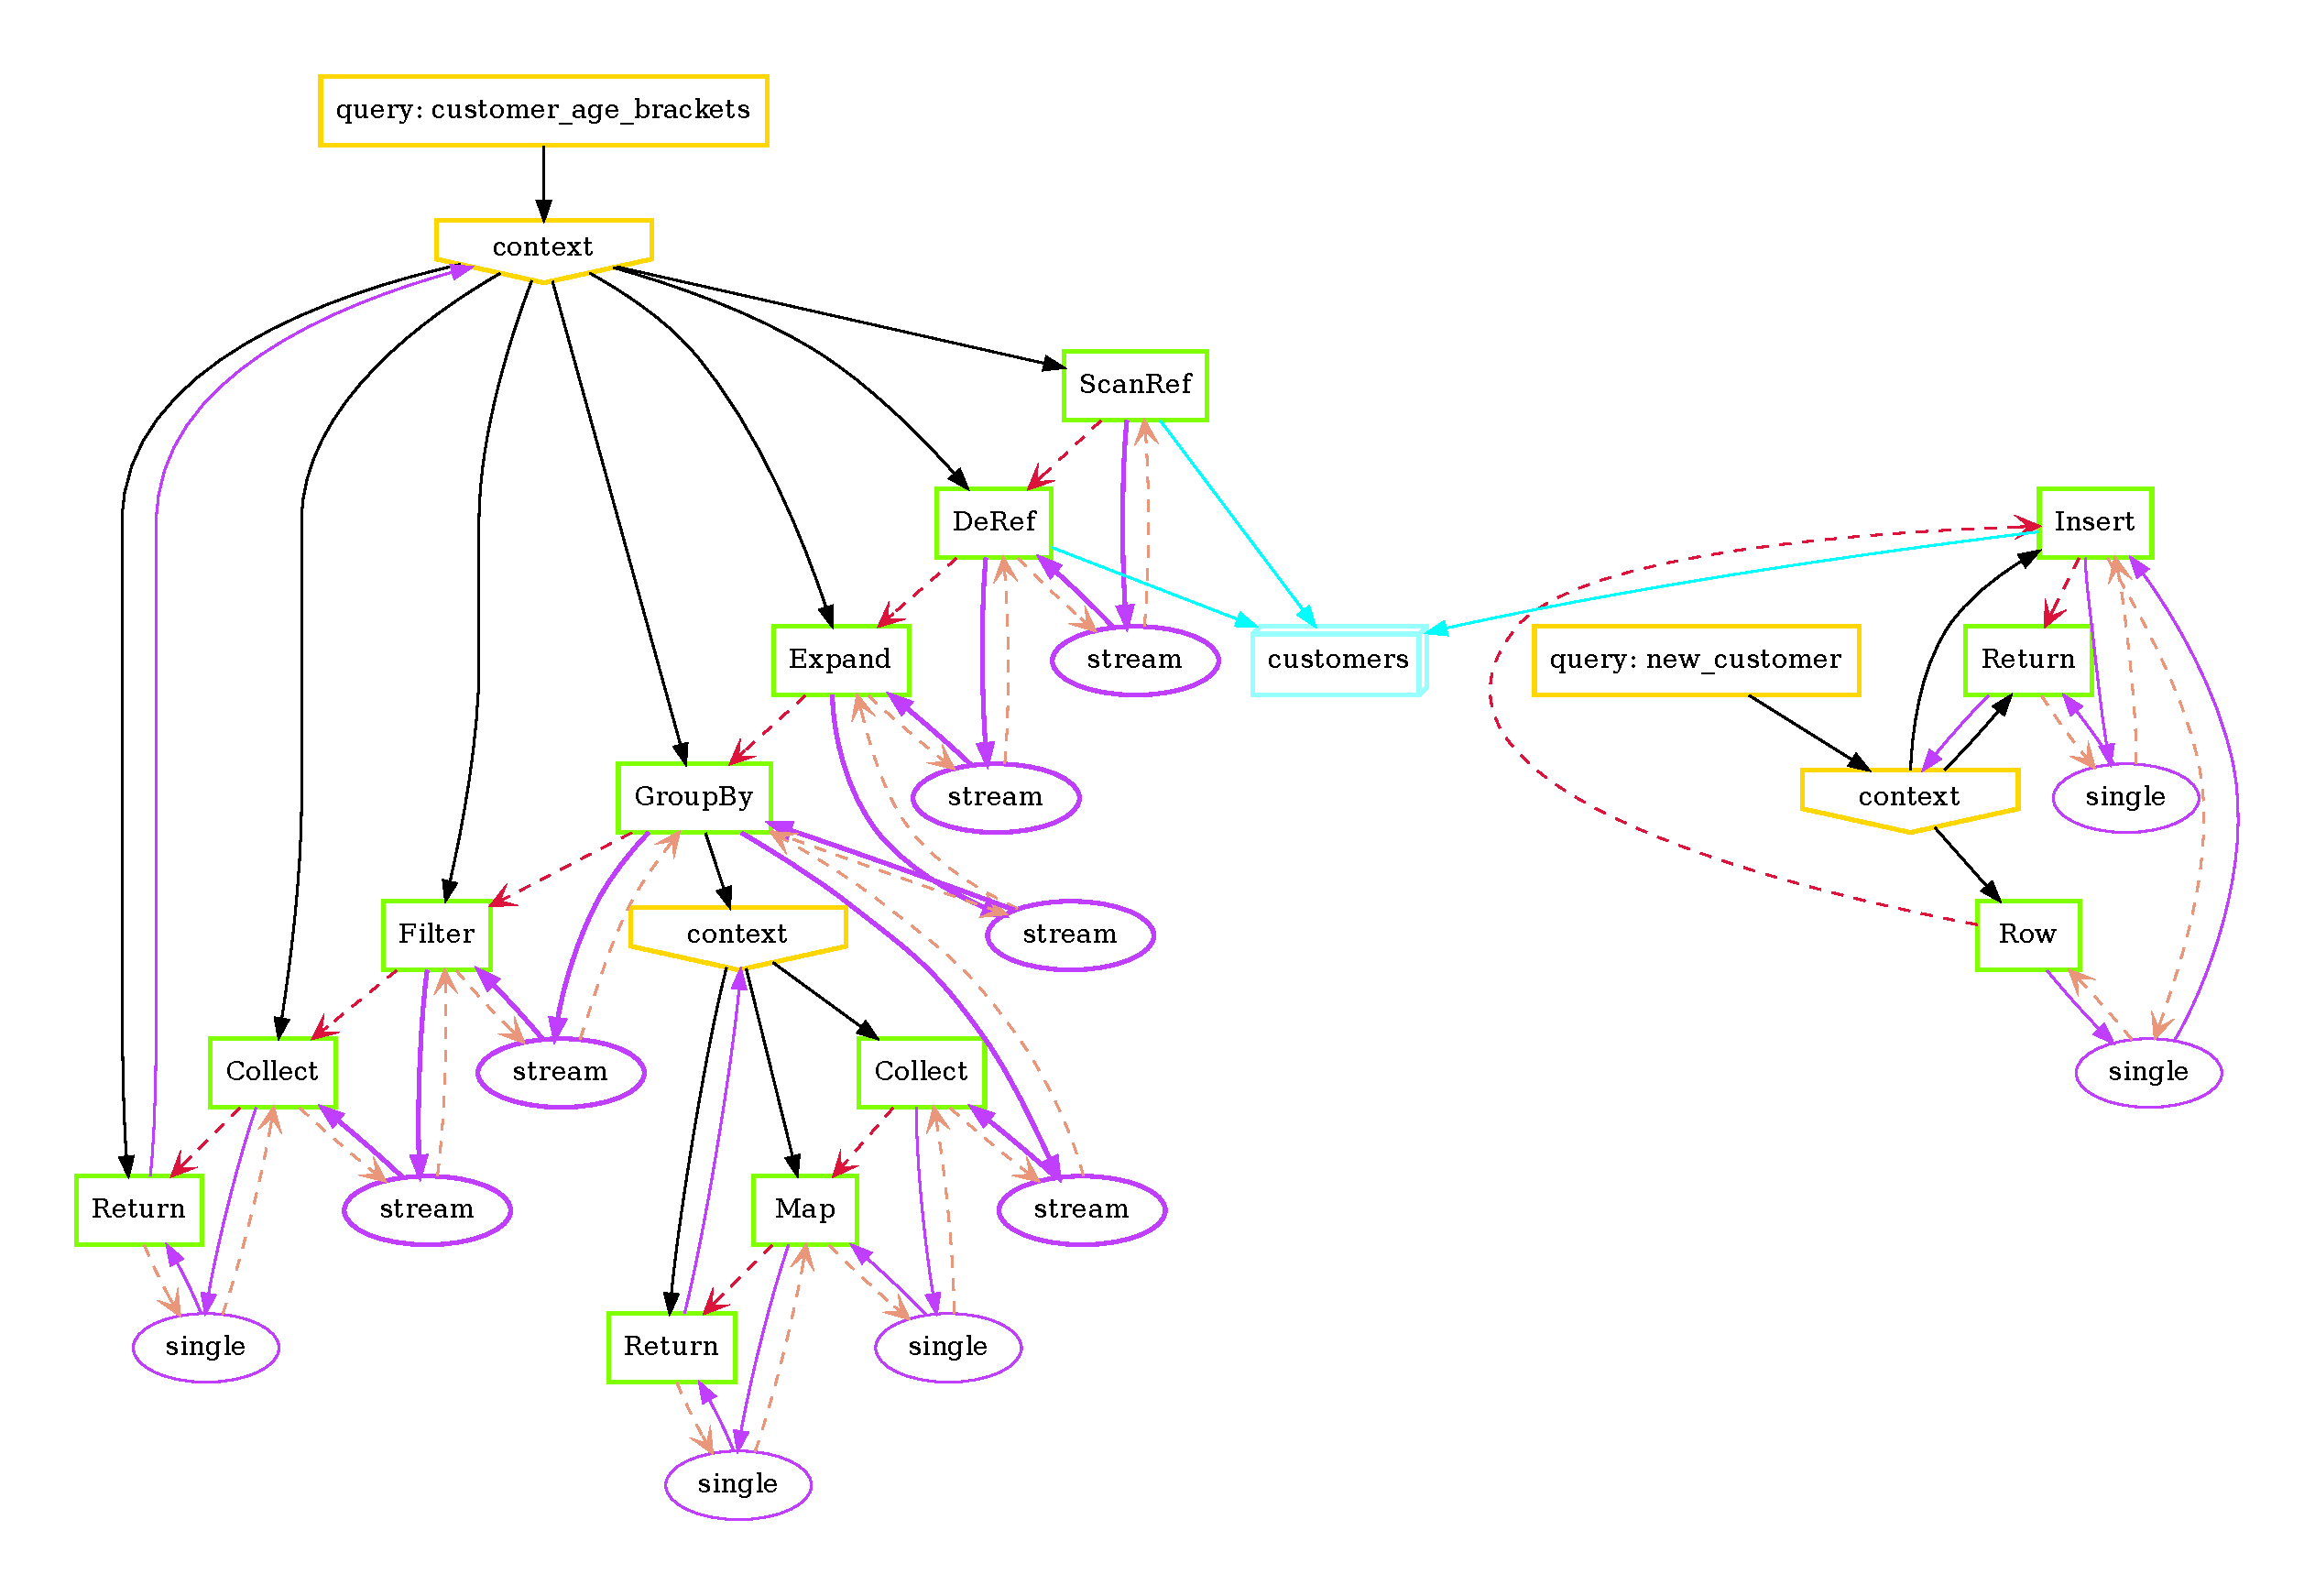
\includegraphics[width=\textwidth]{implementation/diagrams/code.pdf}
    \caption{A plan vizualisation generated at compile time}
\end{figure}


\section{Code Generation}
\subsection{Quasi-quoting}
Rather than manually generating tokenstreams, the \mintinline{rust}{quote!} macro can be used to generate tokenstreams of quasi-quotes. For example the below code is extracted from the \mintinline{rust}{Interface} backend.
\begin{minted}{rust}
quote! {
    if #some_tokenstream {
        #other_tokenstream;
    }
}
\end{minted}
Iteration patterns can be used to extract from iterators (such as vectors of objects implementing the \mintinline{rust}{quote::ToToken} trait).
\begin{minted}{rust}
quote!{ #(#some_statements;)* }
\end{minted}

\begin{futurebox}{Optimising usage of quote}
    In part as a result of the 174 invocations of quote from the pulpit table generation library, from-fresh compilation times for\mintinline{rust}{pulpit_gen} are very slow, and require significant memory ($\approx 6$GB on fresh compile).
    More work needs to be done in optimising this \& emDB's from-fresh build times in general.
\end{futurebox}
\subsection{Serialized Backend}
\begin{center}
    \begin{tabular}{l p{.8\textwidth}}
        \textbf{Serialized Isolation} & The generated database object has no special support for concurrency. It is safe to run concurrent readonly queries (enforced by rust). Mutation can be supported by wrapping the database in a lock.                                      \\
        \textbf{Limited Concurrency}  & Each operator is evaluated in the order they appear in the emQL code. The default operator implementation is not parallel, however an inefficient parallel implementation exists \& compiles.                                              \\
        \textbf{Human Readable}       & The generated rust code is human readable, and can be formatted and output to a separate file at compile time for debugging.                                                                                                               \\
        \textbf{Configurable}         & Table selection and operator implementation are configurable from the emQL \mintinline{rust}{impl} declaration.                                                                                                                            \\
        \textbf{Interface Support}    & The serialized backend can optionally implement a trait for the emQL schema, as is generated by the \mintinline{rust}{Interface} backend, this makes generic tests and benchmarks possible, and is how this report's evaluation was built. \\
    \end{tabular}
\end{center}
\begin{futurebox}{Parallel Queries}
    There are three potential avenues for parallelism in Serialized generated queries.
    \begin{enumerate}
        \setlength\itemsep{0em}
        \item Parallelism between queries.
        \item Parallelism inside operators.
        \item Parallelism in applying operators.
    \end{enumerate}
    The latter is feasable within the current code generation, the generation of expressions \& closures for user expressions (capturing variables from context) is separate from the application of operators to dataflows. So the latter can be re-ordered and parallelised.
    \begin{itemize}
        \setlength\itemsep{0em}
        \item Some extra analysis to ensure accesses to the same tables are synchronised is required within operators, and to maintain observably serial execution between queries.
    \end{itemize}
\end{futurebox}

\subsection{Operator Implementation}
\begin{center}
    \begin{tabular}{l p{.42\textwidth} p{.42\textwidth}}
                             & \textbf{Pull Based/Volcano Processing}                                                                                                                                & \textbf{Push Based/Bulk Processing}                                                                               \\
        \textbf{Description} & Operators pull tokens from input operators.                                                                                                                           & Operators push buffers of tokens to output operators.                                                             \\
        \textbf{Evaluation}  & Lazy                                                                                                                                                                  & Strict                                                                                                            \\
        \textbf{Advantages}  & Keeps values in registers between operators.                                                                                                                          & Code generation for push operators is considerably simpler (Operator takes immediate inputs and assigns outputs). \\
        \textbf{Weakness}    & large number of calls (typically virtual for runtime physical plan generation) and with complex control flow (degrades branch predictor and code locality in icache). & Requires materialising results after every operator.                                                              \\
    \end{tabular}
\end{center}
The minister crate provides the interface for operators, including various maps, filters, joins and buffering. In order to provide a flexible interface that allows \mintinline{rust}{impl trait}
types for streams and single values, in the absence of associated trait items for traits, minister uses a macro to define new traits for operators.
\\
\\ For example the trait generation specifies the filter operation as:
\begin{minted}{rust}
fn filter<Data>(stream: stream!(Data), predicate: impl Fn(&Data) -> bool + Send + Sync) -> stream!(Data)
where
    Data: Send + Sync; 
\end{minted}
For example the default operator implementation for \mintinline{rust}{Serialized} (\mintinline{rust}{Iter}) is defined using the trait generated by:
\begin{minted}{rust}
macro_rules! single { ($data:ty) => { $data }; }
macro_rules! stream { ($data:ty) => { impl Iterator<Item = $data> }; }
super::generate_minister_trait! { IterOps }
\end{minted}
The \mintinline{rust}{Iter} implementation makes use of the rust iterators, whicn are lazily evaluated, monomorphised (no virtuals, can be inlined) streams of data.
\begin{enumerate}
    \setlength\itemsep{0em}
    \item Operators appear push based, \mintinline{rust}{let output = Iter::map(input)}. This makes code generation simple.
    \item However, the \mintinline{rust}{input} and \mintinline{rust}{output} are actually lazy streams, so this is semantically a pull based operator.
    \item At compile time, rust can inline the calls to parent iterators in \mintinline{rust}{input}, converting it into an iteration over the source of the data, directly into a buffer (output). This is physically the same as an optimised push-based system (albeit between the pipeline breaking operators).
\end{enumerate}
This is the same model implemented by hyper\cite{HyperQueryPlan}, though with significantly reduced implementation complexity.
\begin{quote}
    \textit{"\dots data is always pushed from one pipeline-breaker into another
        pipeline-breaker. Operators in-between leave the tuples in
        CPU registers and are therefore very cheap to compute."}
    \\ \vspace{0.5cm}
    \hfill -- \textit{Efficiently Compiling Efficient Query Plans
        for Modern Hardware\cite{HyperQueryPlan}}
\end{quote}
Additionally the rust compiler performs special optimisation for iterators. Specifically in-place-collect for vectors\cite{RustInPlaceCollect}.
This can remove the cost of allocating the output buffer, by reusing the same allocation as the input.
\\
\\ \begin{minipage}{.5\textwidth}
    \textbf{Iterator}
    \begin{minted}{rust}
fn op<I,O>(values: Vec<I>, f: impl Fn(I) -> O)
 -> Vec<O> {
    values
        .into_iter()
        .map(f)
        .collect()
}

    \end{minted}
\end{minipage} \hfill \begin{minipage}{.5\textwidth}
    \textbf{Loop}
    \begin{minted}{rust}
fn op<I,O>(values: Vec<I>, f: impl Fn(I) -> O) 
-> Vec<O> {
    let mut result = Vec::with_capacity(values.len());
    for item in values {
        result.push(f(item));
    }
    result
}
    \end{minted}
\end{minipage}
\begin{figure}[h!]
    \centering
    \begin{tabular}{l l l}
                                              & \textbf{Iters} & \textbf{Loops} \\
        \textbf{Calls to divan AllocProfiler} & 0              & 1              \\
    \end{tabular}
    \caption{Allocations for each implementation when benchmarked with the Divan AllocProfiler}
\end{figure}
\begin{figure}[h!]
    \centering
    \vspace{-0.4em}
    \resizebox{\textwidth}{!}{\input{evaluation/_graphs/iterators.pgf}}
    \caption{Mapping sum onto tuples (using standard allocator)}
\end{figure}

\section{Additional Libraries}
\subsection{Enumtrait}
Many of the data structures inside emDB are represented as rust \mintinline{rust}{enum}s.
This allows for easy pattern matching, but makes implementing traits tedious.
\begin{itemize}
    \setlength\itemsep{0em}
    \item Enumtrait uses tokens from \mintinline{rust}{enum} and \mintinline{rust}{trait} definitions to implement traits on enums of data types that implement the trait.
    \item Boilerplate for type $\to$ \mintinline{rust}{enum} type conversion is also generated.
\end{itemize}
There are existing libraries for this, such as \mintinline{rust}{enum_dispatch}, however this relies on
communication between proc macro invocations at compile time through static data structures.
\begin{itemize}
    \setlength\itemsep{0em}
    \item Significant complexity to cope with ordering of invocations (ordering is undefined by rust).
    \item Needs to tokens types to strings (loosing span information) while communicating (\mintinline{rust}{TokenStream} types are special and cannot be shared between threads).
\end{itemize}


Enumtrait solves the procedural macro communication issue, by generating new \mintinline{rust}{macro_rules!} definitions
as callbacks containing stores of tokens. AS the definition $\to$ use of macros is ordered, this allows communication including tokens and their spans intact.

\begin{minted}{rust}
struct Bar { common_field: usize }
struct Bing { common_field: usize, other_field: String }

#[enumtrait::quick_enum]
#[enumtrait::store(foo_macro_store)]
enum Foo {
    Bar,
    Bing,
}

#[enumtrait::store(foo_trait_store)]
trait FooTrait {
    const BAZ: usize;
    fn foo(&self) -> usize;
}

impl FooTrait for Bar {  
    const BAZ: usize = 1;
    fn foo(&self) -> usize { self.common_field }
}
impl FooTrait for Bing { 
    const BAZ: usize = 2; 
    fn foo(&self) -> usize { self.common_field }
}

#[enumtrait::impl_trait(foo_trait_store for foo_macro_store)]
impl FooTrait for Foo {
    const BAZ: usize = 42;
}

fn check(f: Foo) -> usize { f.foo() }
\end{minted}

